\documentclass[fontsize=14pt,a4paper]{scrartcl}
%\linespread{1.3}
\usepackage[left=3cm, right=2cm, top=2cm, bottom=3cm]{geometry}
\usepackage[utf8]{inputenc}
\usepackage[english,russian]{babel}
\usepackage{indentfirst}
\usepackage{misccorr}
\usepackage{graphicx}
\usepackage{amsmath}
\DeclareGraphicsExtensions{.pdf,.png,.jpg}
\usepackage{url}
\usepackage{listings}
\parindent=1.25cm
\def\labelitemi{--}

%\lstset{frame=tb,language=С,showstringspaces=false,columns=flexible,breaklines=true,breakatwhitespace=true,tabsize=4,aboveskip=3mm,belowskip=3mm}

%\usepackage{listings}
%\usepackage{xcolor}

\lstdefinestyle{sharpc}{language=[Sharp]C, frame=lr, rulecolor=\color{blue!80!black}}



\begin{document}
\title{Параллельные вычисления в задаче оптимизации структуры 3D моделей}
\author{Самсонов Андрей Федорович}
\date{\today}

\titlepage
\begin{center}
МИНОБРНАУКИ РОССИИ\\
\vspace{0.5cm}
Федеральное государственное бюджетное образовательное\\
учреждение высшего профессионального образования\\
«Ярославский государственный университет им. П.Г. Демидова»\\
\vspace{0.5cm}
{\bf Кафедра математического моделирования}\\
\end{center}

\begin{flushright}
"Допустить к защите"\\
Зав. кафедрой,\\
доктор ф.-м.н., профессор\\
\underline{\phantom{aaaaaaaaaaaa}} С. А. Кащенко\\
«
\underline{\phantom{aaa}}
»
\underline{\phantom{aaaaaaaaaaaaa}} 2015 г.\\
\end{flushright}

\begin{center}
\vspace{3cm}
Выпускная квалификационная работа бакалавра\\
\vspace{0.5cm}
Параллельные вычисления в задаче оптимизации структуры 3D моделей\\
\vspace{3cm}
\end{center}

\begin{flushright}
Научный руководитель\\
кандидат физ.-мат. наук, доцент\\
\underline{\phantom{aaaaaааaaaaaa}} Д. С. Глызин\\
«
\underline{\phantom{aaa}}
»
\underline{\phantom{aaaaaaaaaaaaa}} 2015 г.\\
\vspace{0.5cm}
%Студент группы ПМИ-42БО
\underline{\phantom{aaaaaaaaaaa}} А. Ф. Самсонов\\
«
\underline{\phantom{aaa}}
»
\underline{\phantom{aaaaaaaaaaaaaa}}2015 г.\\
\vspace{2.5cm}
\begin{center}
Ярославль 2015 г.
\end{center}
\end{flushright}
\titlepage
\clearpage
\begin{center}\Large{Реферат}\end{center}
Объем 25 с., 8 рис., 3 табл., 9 источников, 4 прил.\newline
{\bf Параллельные вычисления, самозатенение, ambient occlusion, GPGPU, OpenCL, оптимизация 3D моделей.}\newline
	
Объектом исследования являются алгоритмы расчета самозатенения 3D моделей с использованием параллельных вычислений.

	Цель работы – разработка программного комплекса для расчета самозатенения и удаления внутренней геомтерии.

	В процессе работы были найдены способы расчета коэффициента самозатенения, а так же оптимизировано время его расчета.

	В результате была созданна программа, способная расчитать самозатенение для моделей любого размера (вплоть до нескольких миллионов полигонов) за приемлимое время.
	
На данном этапе программа может применятся для подготовки моделей к 3D печати.
\setcounter{page}{2} 
\clearpage\tableofcontents
\clearpage
\addcontentsline{toc}{section}{\rm{\Large{Введение}}}
3D-принтер — это периферийное устройство, использующее метод послойного создания физического объекта по цифровой 3D-модели. В настоящее время это очень быстроразвивающаяся область, имеющая массу применений и позволяющая изготавливать объекты, которые невозможно создать другими способами. Существует несколько технологий, с помошью которых происходит создание итогового объекта

\begin{itemize}
\item Лазерная стереолитография
\item Лазерное сплавлени
\item Ламинирование
\item Застывание материала при охлаждении
\item Полимеризация фотополимерного пластика под действием ультрафиолетовой лампы
\item Склеивание или спекание порошкообразного материала
\end{itemize}

Все варианты печати предусматривают использование некоторой трехменой модели для создания программы печати, например на кафедре математического моделирования ЯРГУ, некоторые модели, печатающиеся там, представляют из себя визаулизацию некоторых математических функций. При задании модели функцией получается модель теоретически неограниченной точности, но зачастую в такой модели образуется большое число полигонов, которые находятся внутри модели и не имеют смысла как для печати, так и для рендеринга. В настоящей работе целью была разработка программы, предназначенной для оптимизации таких моделей т.е. отсечения геометрии, которая находится внутри модели, будем называть такую геометрию внутренней.

\clearpage
\section{Входные данные}
\subsection{STL}
STL (от англ. stereolithography) -- открытый формат файла используемый для хранения 3D моделей и является основной для большинства 3D принтеров, за исключением внутренних форматов, которые рассматривать не будем, т.к. число этих форматов постоянно увеличивается и, фактически, большинство разработчиков аппаратуры 3D печати создают собственные форматы под свои нужды. Информация в STL может хранится как в текстовом, так и в двоичном виде. Вся геометрия задается в виде наборов точек, составляющих треугольник и соответствующую им нормаль, которая не используется при печати. Этот формат был выбран основным форматом для программы по причине его простоты, достаточности для целей не цветной печати и большой распространенности. Формат используется как для загрузки моделей, так и для сохранения.
\subsection{Obj}
Более продвинутый формат, чем STL, разработанный в Wavefront Technologies. Формат так-же является открытым и очень распространен, поддерживается большинством современных 3D редакторов, но в отличии от STL имеет более расширенные возможности, такие как текстурные координаты, нетреугольные полигоны, а так же дополнительные файлы, описывающие материалы, используемые для текстурирования. Используется в проекте для загрузки моделей, выбран по причине простоты и большой распространенности.

\clearpage

\section{Расчет досягаемости геометрии}\label{main_part}

Элементы поверхности. Первым шагом алгоритма будет упрощение данных о геометрии. Упрощение сводит каждый полигон к окружности, имеющей координаты центра, нормаль и площадь, оно позволит сильно упростить расчеты того, насколько одна из поверхностей затеняет другую. Центром окружности является усредненное значение координат всех точек полигона.
\begin{equation}
	\sum_{i=0}^{n} x_i / n
\end{equation}

Нормаль вычисляется по трем любым точкам ($a$, $b$, $c$) по следующей формуле:
\begin{equation}\begin{split}
	w = {(c-a) \times (b-a)} \\
	n = w \cdot 1 / \sqrt{\sum_{i=0}^{n} {w_i^2}}
\end{split}\end{equation}

Площадь треугольника вычислим по формуле Герона.
\begin{equation}\begin{split}
	p= {{a+b+c}\over{2}} \\
	S=\sqrt{p(p-a)(p-b)(p-c)}
\end{split}\end{equation}

\begin{figure}[h]
	\center
	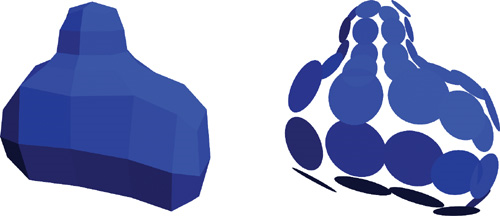
\includegraphics[width=0.5\textwidth]{14_ambient_occlusion_02}
	\caption{Перевод полигонов в диски той же площади}\label{fig:ao02}
\end{figure}
Ambient occlusion -- полезная техника для затенения объектов, которая используется в современной графике. Благодаря ambient occlusion получаются мягкие тени за счет затемнения поверхностей, которые частично видны с некоторой внешней точки. Эта техника также включает в себя расчет коэффициента досягаемости полигона к окружению, или, другими словами, число обратное числу пересечений его с другими полигонами в полусфере перед первым.

Досягаемость для каждого элемента может быть вычислена, как 1 минус доля затенения этого жлемента остальными. Быдем называть элемент, на который падает тень ресивером, а элемент бросающий тень  -- эммитером. Для расчетов количества тени, которая бросается эммитером на ресивер используется формула, основанная на телесном угле для ориентированного диска 


\begin{equation}
	1-{{r\cos{\Theta_E \max(1, 4\cos{\Theta_R})}}\over{\sqrt{{A\over\pi} + r^2}}}
	\label{em_rec}
\end{equation}
Где $А$ -- площадь эммитера\\
$E$ -- эммитер\\
$R$ -- ресивер\\
$RE$ -- отрезок, соединяющий центры дисков\\
$r$ -- длина отрезка RE, расстояние между дисками\\
$\Theta_R$ -- угол между нормалью ресивера и отрезком ER\\
$\Theta_E$ -- угол между нормалью эммитера и отрезком ER\\

\begin{figure}[h]
	\center
	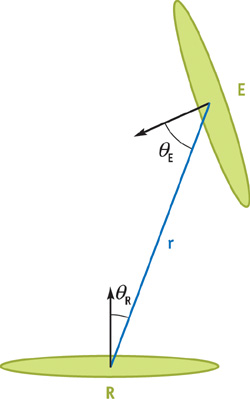
\includegraphics[width=0.3\textwidth]{14_ambient_occlusion_03}
	\caption{визуализация расположения эммитера и ресивера и эелементов уравнения \ref{em_rec}}\label{fig:ao03}
\end{figure}



\clearpage
\addcontentsline{toc}{section}{\rm{\Large{Заключение}}}
В результате было создано приложение, которое может загружать, сохранять и отображать любые модели в формате STL и Obj, а так же выполнять расчет самозатенения и отсечения геометрии, тем самым упрощая структуру модели непосредственно перед ее печатью или последующим рендером.Одной из целей настоящей работы являлось сравнение выгоды от применения параллельных вычислений, в.т.ч. с применением GPU. Применение GPU позволило ускорить скорость работы алгоритма примерно в 40 раз. Производительность оказалась вполне достаточной для разового расчета, для больших моделей, порядка четырех миллионов полигонов, производится в течении 8 минут на видеокарте бюджетного уровня. Для небольших моделей (несколько сотен тысяч полигонов) расчет производится практически мгновенно.
\clearpage
\begin{thebibliography}{00}
\bibitem{book1} GPU Gems 2: Programming Techniques For High-Performance Graphics And General-Purpose Computation. Matt Pharr, Randima Fernando. Pearson Addison Wesley Prof, 2005  -Всего страниц: 814
\bibitem{book11} Christensen, P. H. 2002. Note \#35: Ambient Occlusion, Image-Based Illumination, and Global Illumination.
\bibitem{book12} Chunhui, M., Jiaoying, S., and Fuli, W. 2004. Rendering with Spherical Radiance Transport Maps. Computer Graphics.
\bibitem{book13} Deering, M., Winner, S., Schediwy, B., Duffy, C., and Hunt, N. 1988. The Triangle Processor and Normal Vector. Shader: A VLSI System for High Performance Graphics.
\bibitem{book14} Iones, A., Krupkin, A., Sbert, M., and Zhukov, S. 2003. Fast, Realistic Lighting for Video Games.
\bibitem{book15} Kautz, J., Lehtinen, J., and Aila, T.  2004.  Hemispherical Rasterization for Self-Shadowing of Dynamic Objects.
\bibitem{bool16} Sattler, M., Sarlette, R., Zachmann, G., and Klein, R., 2004. Hardware-accelerated ambient occlusion computation. To appear in the proceedings of International Fall Workshop on Vision, Modeling, and Visualization 2004.
\bibitem{book2} \url{http://www.cadcamcae.lv/hot/STL_n23_p64.pdf}
\bibitem{book4} \url{http://www.fabbers.com/tech/STL_Format}
\end{thebibliography}

\clearpage
\Large{Приложение А}
\begin{lstlisting}
public void RecalcNormals()
{
    for (int i = 0; i < Verteces.Count; i += 3)
    {
        var a = Verteces[i].Position;
        var b = Verteces[i + 1].Position;
        var c = Verteces[i + 2].Position;
        var normal = Vector3.Normalize(
              Vector3.Cross(c - a, b - a));
        var i0 = Verteces[i];
        var i1 = Verteces[i + 1];
        var i2 = Verteces[i + 2];

        i0.Normal = i1.Normal = i2.Normal = 
            normal;
        Verteces[i] = i0;
        Verteces[i + 1] = i1;
        Verteces[i + 2] = i2;
    }
    FlipNormals();
}
public void FlipNormals() {
    for (int i = 0; i < Verteces.Count; i++) {
        var vertex = Verteces[i];
        vertex.Normal *= -1;
        Verteces[i] = vertex;
    }
}
\end{lstlisting}


\clearpage
\Large{Приложение Б}
\begin{lstlisting}
__kernel void floatSquareDivPi(
    __global float * vx, 
    __global float * vy, 
    __global float * vz,
    __global float * nx, 
    __global float * ny, 
    __global float * nz, 
    __global float * a, 
    __global float * s)
{ 
    int i = get_global_id(0)*3;
    float3 vec1 = (float3)(vx[i], 
              vy[i], vz[i]); 
    float3 vec2 = (float3)(vx[i+1], 
               vy[i+1], vz[i+1]); 
    float3 vec3 = (float3)(vx[i+2], 
              vy[i+2], vz[i+2]); 
    float A = distance(vec1, vec2);
    float B = distance(vec2, vec3);
    float C = distance(vec1, vec3);
    float S = (A + B + C) / 2.0f;
    float sq = sqrt(S * (S - A) * 
            (S - B) * (S - C)) / M_PI;
    s[i] = s[i+1] = s[i+2] = sq;
}

float ElementShadow(float3 v, 
        float rSquared, 
        float3 receiverNormal, 
        float3 emitterNormal, 
        float emitterArea) {
    return (1.0f - rsqrt(emitterArea/
               rSquared + 1.0f)) *
    clamp(dot(emitterNormal, v), 
              0.0f, 1.0f) *
    clamp(4.0f * dot(receiverNormal, 
              v), 0.0f, 1.0f);
}

__kernel void floatAO(
               __global float * vx, 
               __global float * vy, 
               __global float * vz,
	    __global float * nx, 
               __global float * ny, 
               __global float * nz,
	    __global float * a, 
               __global float * s, 
               long from)
{ 
    int i = from + get_global_id(0)*3;
    float res = 0.0f;
    float3 v = (float3)(0, 0, 0);
    float d2 = 0;
    float value = 0;
    for(int j = 0; j<count;j+=3){
        v = (float3)(vx[j], vy[j], vz[j]) - 
               (float3)(vx[i], vy[i], vz[i]);
        d2 = dot(v, v) + 1e-16;                            
        v *= rsqrt(d2);
        value = ElementShadow(v, d2, 
        (float3)(nx[i], ny[i], nz[i]), 
        (float3)(nx[j], ny[j], nz[j]), 
        s[j]);
        res += value;
    }                        
 a[i] = a[i+1] = a[i+2] = 1.0f - res;
}
\end{lstlisting}

\clearpage
\Large{Приложение В} \newline
\begin{table}[h]
\begin{tabular}{|cc|}
00:01:43.419 & \\
00:01:44.241  & \\
00:01:32.125  & \\
00:01:44.158  & \\
00:01:37.423  & \\
\end{tabular}
Среднее: 00:01:40.2732
\end{table}


\begin{table}[h]
\begin{tabular}{|cc|}
00:00:30.205 & \\
00:00:29.944  & \\
00:00:30.072  & \\
00:00:29.832  & \\
00:00:30.341  & \\
\end{tabular}
Среднее: 00:00:30.0788
\end{table}


\begin{table}[h]
\begin{tabular}{|cc|}
00:00:02.527 & \\
00:00:02.502  & \\
00:00:02.509  & \\
00:00:02.549  & \\
00:00:02.511  & \\
\end{tabular}
Среднее: 00:00:02.5196
\end{table}

\end{document}

